\PassOptionsToPackage{unicode=true}{hyperref} % options for packages loaded elsewhere
\PassOptionsToPackage{hyphens}{url}
%
\documentclass[11,]{article}
\usepackage{lmodern}
\usepackage{amssymb,amsmath}
\usepackage{ifxetex,ifluatex}
\usepackage{fixltx2e} % provides \textsubscript
\ifnum 0\ifxetex 1\fi\ifluatex 1\fi=0 % if pdftex
  \usepackage[T1]{fontenc}
  \usepackage[utf8]{inputenc}
  \usepackage{textcomp} % provides euro and other symbols
\else % if luatex or xelatex
  \usepackage{unicode-math}
  \defaultfontfeatures{Ligatures=TeX,Scale=MatchLowercase}
\fi
% use upquote if available, for straight quotes in verbatim environments
\IfFileExists{upquote.sty}{\usepackage{upquote}}{}
% use microtype if available
\IfFileExists{microtype.sty}{%
\usepackage[]{microtype}
\UseMicrotypeSet[protrusion]{basicmath} % disable protrusion for tt fonts
}{}
\IfFileExists{parskip.sty}{%
\usepackage{parskip}
}{% else
\setlength{\parindent}{0pt}
\setlength{\parskip}{6pt plus 2pt minus 1pt}
}
\usepackage{hyperref}
\hypersetup{
            pdfborder={0 0 0},
            breaklinks=true}
\urlstyle{same}  % don't use monospace font for urls
\usepackage[margin=1in]{geometry}
\usepackage{graphicx,grffile}
\makeatletter
\def\maxwidth{\ifdim\Gin@nat@width>\linewidth\linewidth\else\Gin@nat@width\fi}
\def\maxheight{\ifdim\Gin@nat@height>\textheight\textheight\else\Gin@nat@height\fi}
\makeatother
% Scale images if necessary, so that they will not overflow the page
% margins by default, and it is still possible to overwrite the defaults
% using explicit options in \includegraphics[width, height, ...]{}
\setkeys{Gin}{width=\maxwidth,height=\maxheight,keepaspectratio}
\setlength{\emergencystretch}{3em}  % prevent overfull lines
\providecommand{\tightlist}{%
  \setlength{\itemsep}{0pt}\setlength{\parskip}{0pt}}
\setcounter{secnumdepth}{0}
% Redefines (sub)paragraphs to behave more like sections
\ifx\paragraph\undefined\else
\let\oldparagraph\paragraph
\renewcommand{\paragraph}[1]{\oldparagraph{#1}\mbox{}}
\fi
\ifx\subparagraph\undefined\else
\let\oldsubparagraph\subparagraph
\renewcommand{\subparagraph}[1]{\oldsubparagraph{#1}\mbox{}}
\fi

% set default figure placement to htbp
\makeatletter
\def\fps@figure{htbp}
\makeatother

\usepackage{ctex}
\usepackage{xcolor}
\usepackage{fancyhdr}
\usepackage{sectsty}
\definecolor{glaucous}{rgb}{0.38, 0.51, 0.71}
\definecolor{lavenderblush}{rgb}{1.0, 0.94, 0.96}
\usepackage{enumitem}% http://ctan.org/pkg/enumitem
\usepackage[empty]{fullpage}% http://ctan.org/pkg/fullpage
\usepackage{color}% http://ctan.org/pkg/color
\usepackage{hyperref}% http://ctan.org/pkg/hyperref
\usepackage{geometry}
\usepackage{blindtext}
\textwidth 6.75in
\textheight 8.5in
\oddsidemargin -.25in
\evensidemargin -.25in
\topmargin -0.5in

\title{\textcolor{glaucous}{新冠早报}}
\author{\textcolor{glaucous}{第六期 3月28日}}
\date{}

\begin{document}
\maketitle

\newcommand{\resheading}[1]{%
  \noindent\fcolorbox{lavenderblush}{lavenderblush}{\makebox[\dimexpr\textwidth-2\fboxsep-2\fboxrule][l]{\textbf{~#1}}}%
}

\pagestyle{fancyplain}
\lhead{
\includegraphics[height=2cm]{logo.png}}
\rhead{\begin{tabular}[b]{@{}c@{}}中美健康峰会“智援组” 新冠早报组\\ \\ \end{tabular}}

%
  \noindent\fcolorbox{lavenderblush}{lavenderblush}{\makebox[\dimexpr\textwidth-2\fboxsep-2\fboxrule][l]{\textbf{~新闻摘要}}}%

\textless{}\textless{}\textless{}\textless{}\textless{}\textless{}\textless{}
HEAD %

数据源:约翰霍普金斯大学,The COVID Tracking Project

数据截至:北京时间3月27日早7:30

======= \#\# \textcolor{glaucous}{国际}
\textgreater{}\textgreater{}\textgreater{}\textgreater{}\textgreater{}\textgreater{}\textgreater{}
e50667356eea97ad6dc72145894bc27d85d83e33

\textbf{\textcolor{glaucous}{有线电视新闻网(CNN)}}:
\textbf{特朗普签署2万亿美元的经济援助法案}

当地时间3月27日下午4时30分,美国总统特朗普发推文称他签署了美国有史以来金额最大的经济援助法
案(CARES法),该法案总救济金额为2.2万亿美元,将为美国的家庭、工人和企业提供紧急救援。

\textbf{\textcolor{glaucous}{有线电视新闻网(CNN)}} :
\textbf{特朗普签署2万亿美元的经济援助法案}

当地时间3月27日下午4时30分,美国总统特朗普发推文称他签署了美国有史以来金额最大的经济援助法
案(CARES法),该法案总救济金额为2.2万亿美元,将为美国的家庭、工人和企业提供紧急救援。

\hypertarget{section}{%
\subsection{\texorpdfstring{\textcolor{glaucous}{国内}}{}}\label{section}}

\textbf{\textcolor{glaucous}{有线电视新闻网(CNN)}}:
\textbf{特朗普签署2万亿美元的经济援助法案}

当地时间3月27日下午4时30分,美国总统特朗普发推文称他签署了美国有史以来金额最大的经济援助法
案(CARES法),该法案总救济金额为2.2万亿美元,将为美国的家庭、工人和企业提供紧急救援。

%
  \noindent\fcolorbox{lavenderblush}{lavenderblush}{\makebox[\dimexpr\textwidth-2\fboxsep-2\fboxrule][l]{\textbf{~疫情观察}}}%

数据源:约翰霍普金斯大学,The COVID Tracking Project
数据截止至:北京时间3月28日 早4:00

\hypertarget{section-1}{%
\section{\texorpdfstring{\textcolor{glaucous}{一、世界疫情}}{}}\label{section-1}}

截止北京时间3月28日早6:00,全球累计591,802例确诊病例。

\begin{figure}[htbp] 
\centering %图片居中
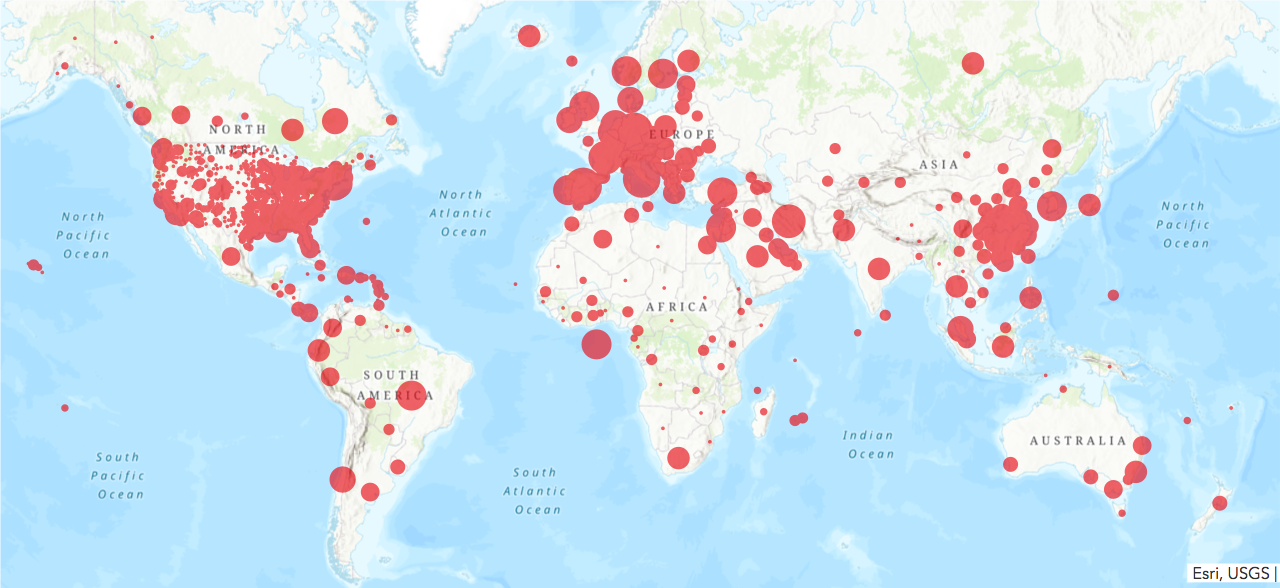
\includegraphics[]{./test/covid1.png} %插入图片,[]中设置图片大小,{}中是图片文件名
\caption{世界疫情分布图 (Global Map of Cumulative Confirmed COVID-19 Cases)} %最终文档中希望显示的图片标题
\label{} %用于文内引用的标签
\end{figure}

\begin{table}[]
\caption{累计确诊前十位国家}
\centering
\resizebox{\textwidth}{!}{%
\begin{tabular}{lllll}
\hline
  & 国家               & 累计确诊病例  & 国家/省份人口     & 粗发病率 \\
  \hline
1 & 美国 United States & 101,567 & 331,002,651 & 31   \\
2 & 意大利 Italy        & 86,498  & 60,461,826  & 143 \\
\hline
\end{tabular}%
}
\end{table}

\begin{minipage}{\textwidth}
        \begin{minipage}[t]{0.5\textwidth}
            \centering
            \begin{tabular}{llll}
            \hline
             & 国家        & 累计死亡病例 & 较昨⽇ \\
            \hline
            1 & 意⼤利 Italy & 9,134  & 919 \\
            2 & 西班⽛ Spain & 4,940  & 575 \\
            \hline
            \end{tabular}
            \makeatletter\def\@captype{table}\makeatother\caption{累计死亡前十位国家}
        \end{minipage}
        \begin{minipage}[t]{0.5\textwidth}
            \centering
            \begin{tabular}{llll}
            \hline
              & 国家         & 当⽇新增病例 & 较昨日  \\
            \hline
            1 & 美国 US      & 17,821 & -237 \\
            2 & 德国 Germany & 6,933  & 318 \\
            \hline
        \end{tabular}
      \makeatletter\def\@captype{table}\makeatother\caption{⽇新增病例前十位国家}
    \end{minipage}
\end{minipage}

\textless{}\textless{}\textless{}\textless{}\textless{}\textless{}\textless{}
HEAD

\textcolor{glaucous}{表1:累计确诊前十位国家}

=======
\textgreater{}\textgreater{}\textgreater{}\textgreater{}\textgreater{}\textgreater{}\textgreater{}
6fbddbd6404aa790eaa5f0496c6a90534dd98d92

\hypertarget{section-2}{%
\section{\texorpdfstring{\textcolor{glaucous}{二、中国与其他疫情严重国家对比}}{}}\label{section-2}}

从累计死亡病例数(表2)来看,全球累计死亡病例数前十国家位次不变。

\begin{figure}[htbp]
\centering  %图片全局居中
\subfigure[累计确诊病例国家趋势图]{
\label{Fig.sub.1}
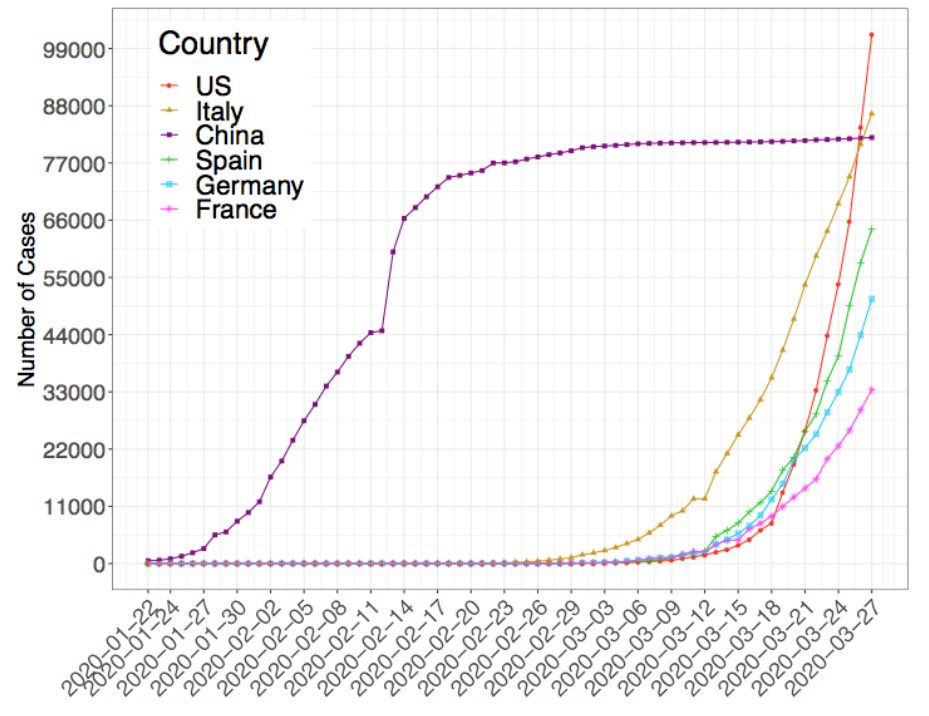
\includegraphics[width=0.45\textwidth]{./test/covid2.png}}
\subfigure[日新增确诊病例国家趋势图]{
\label{Fig.sub.2}
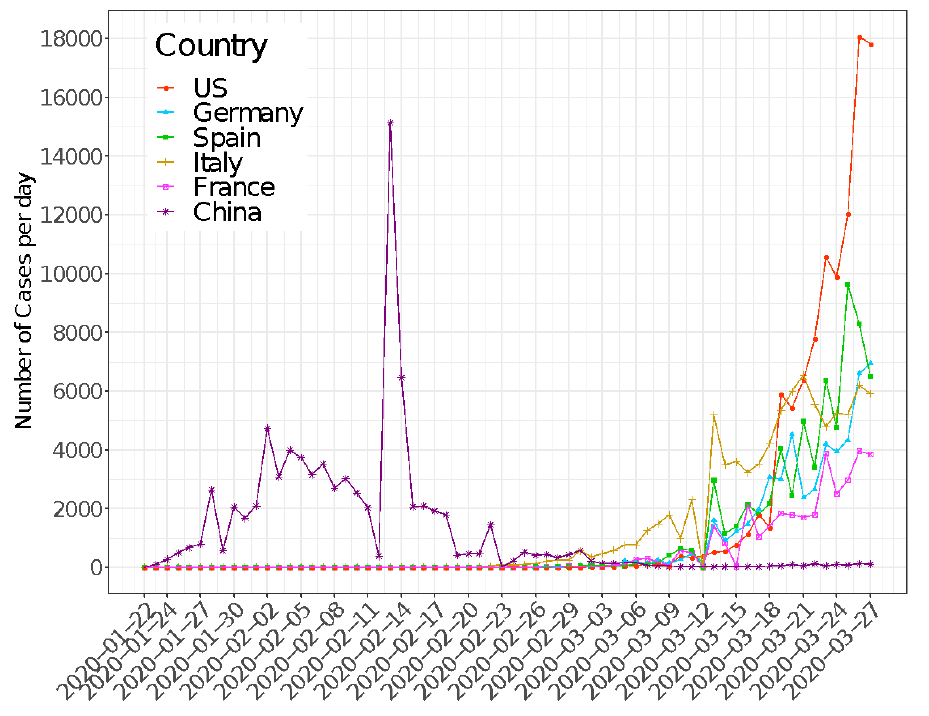
\includegraphics[width=0.45\textwidth]{./test/covid3.png}}
\caption{}
\label{Fig.main}
\end{figure}

\hypertarget{section-3}{%
\section{\texorpdfstring{\textcolor{glaucous}{三、美国疫情}}{}}\label{section-3}}

截至北京时间3⽉28⽇早6:00,
美国共101,567例累计确诊病例,1,581例累计死亡病例。

\begin{figure}[htbp] 
\centering %图片居中
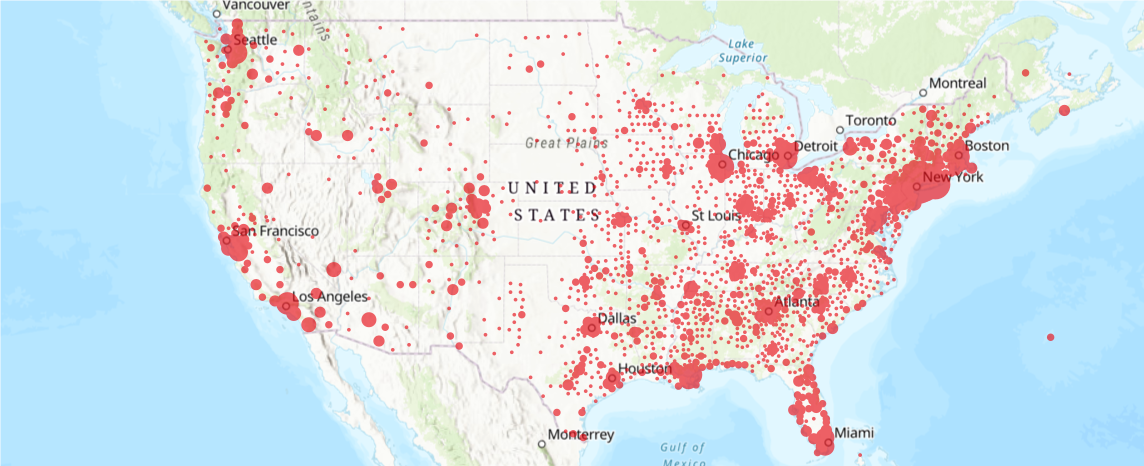
\includegraphics[]{./test/covid4.png} %插入图片,[]中设置图片大小,{}中是图片文件名
\caption{美国本土疫情分布图 (Map of Cumulative Confirmed COVID-19 Cases in Contiguous U.S.)} %最终文档中希望显示的图片标题
\label{} %用于文内引用的标签
\end{figure}

\begin{minipage}{\textwidth}
        \begin{minipage}[t]{0.5\textwidth}
            \centering
            \begin{tabular}{llll}
            \hline
               & 国家/州名   & 累计确诊病例  & 粗发病率 \\
            \hline
           & 美国 US   & 101,567 & 31   \\
         1 & 纽约州 NY  & 44,876  & 231  \\
         2 & 新泽西州 NJ & 8,825   & 99\\
            \hline
            \end{tabular}
            \makeatletter\def\@captype{table}\makeatother\caption{美国累计确诊前十位州}
        \end{minipage}
        \begin{minipage}[t]{0.5\textwidth}
            \centering
            \begin{tabular}{llll}
            \hline
            & 国家/州名   & 当日新增病例 & 全美比率 \\
            \hline
            & 美国 US   & 17821  & 100  \\
          1 & 纽约州 NY  & 7,618  & 43   \\
          2 & 新泽西州 NJ & 1,949  & 11 \\
            \hline
        \end{tabular}
      \makeatletter\def\@captype{table}\makeatother\caption{美国新增确诊前十位州}
    \end{minipage}
\end{minipage}

\begin{figure}[htbp]
\centering  %图片全局居中
\subfigure[美国本土疫情分布图]{
\label{Fig.sub.1}
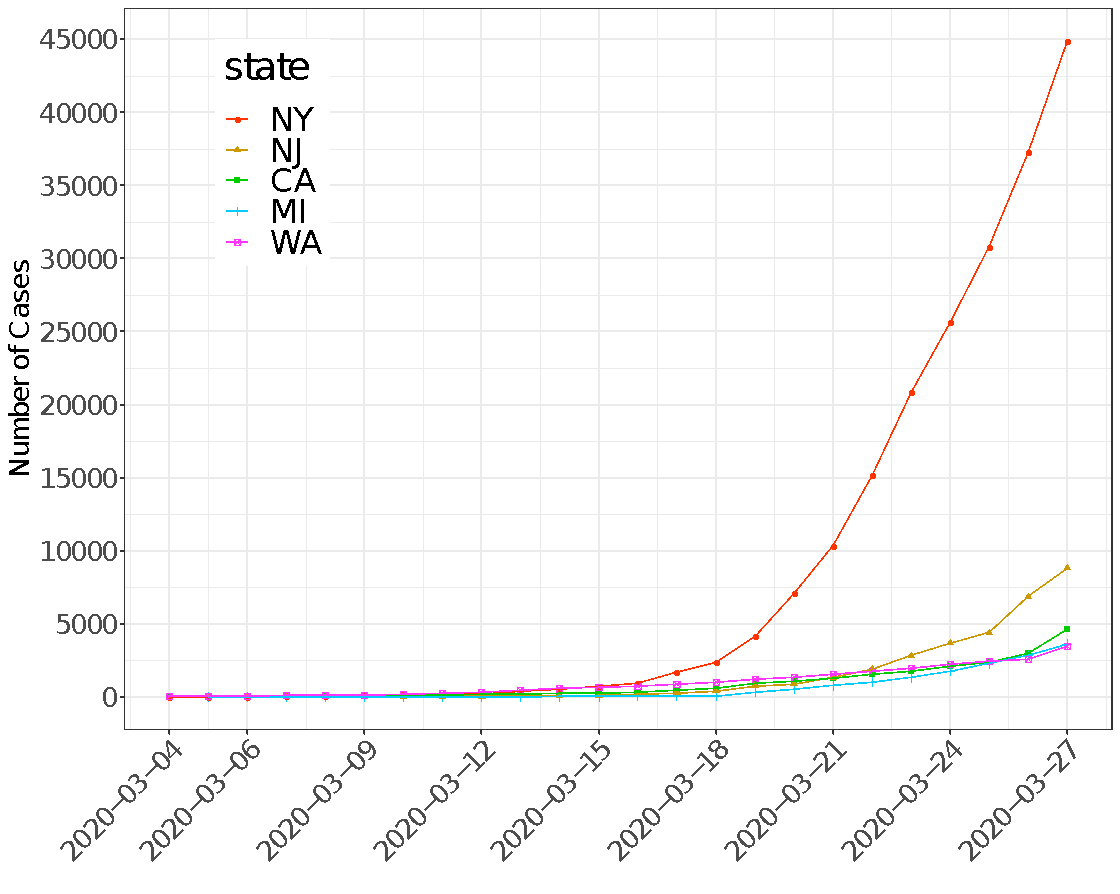
\includegraphics[width=0.45\textwidth]{./test/covid5.png}}
\subfigure[美国累计确诊前五位州趋势图]{
\label{Fig.sub.2}
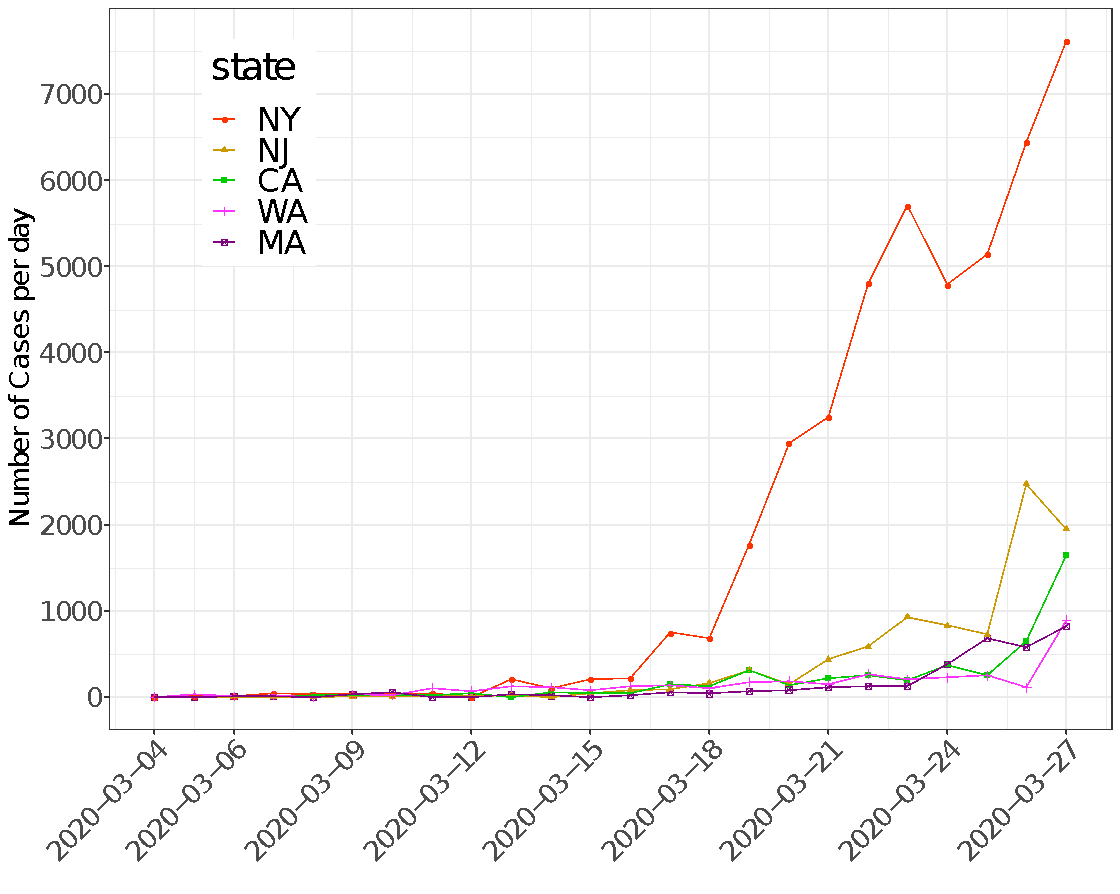
\includegraphics[width=0.45\textwidth]{./test/covid6.png}}
\caption{}
\label{Fig.main}
\end{figure}

\end{document}
